\begin{figure}[h!]
    \begin{center}
        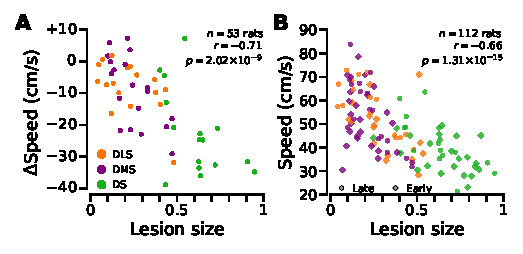
\includegraphics[scale=1]{ch-appendicies/figures/Speed.pdf}
        \caption[Speed-Lesion Size Correlation]
        {\textbf{The running speed negatively correlates with the size of the striatal lesion.}
        \textbf{A)}
        Average change in running speed (speed after lesion~$-$~speed before lesion) versus the lesion size, for all the rats that received a striatal lesion after training (late lesion).
        All speed values were averaged across 5~consecutive sessions before (last 5~sessions before lesion) and after (sessions~\#4 to~\#9, relative to lesion break) lesion.
        \textbf{B)}
        Average running speed versus lesion size for all the animals that underwent surgical lesion of the striatum.
        This dataset ($n=112$ animals) includes animals that underwent striatal lesion after extensive training (Late group, $n=53$, same animals as in panel~A), and animals that underwent lesion before training (Early group, $n=59$ animals).
        Speed was computed as in~A, except that average was done over the last 5 sessions (for both Early and Late groups).
        }
        \label{fig:appendix:spd}
    \end{center}
\end{figure}